\documentclass[hyperref]{beamer}

\usepackage[ngerman]{babel}
\usepackage{pgf,pgfarrows,pgfnodes,pgfautomata,pgfheaps,pgfshade}
\usepackage[utf8]{inputenc}
\usepackage{graphicx}

\usetheme{Frankfurt}

\title{Yaoha}
\subtitle{Yet Another Opening Hours Application}
\author[Hobohm, Reinhardt, Uschok]{Stefan Hobohm, Lutz Reinhardt, Matthias Uschok}
\institute[TU Braunschweig, IBR]{Technische Universität Braunschweig, IBR}

\begin{document}
\frame[plain]{\titlepage}

\frame{
  \frametitle{Outline}
  \tableofcontents
}

\section{Aufgabenstellung}
%\frame{\frametitle{Outline} \tableofcontents[currentsection]}
\subsection{}

\begin{frame}{Probleme unterschiedlicher Öffnungszeiten}
\begin{itemize}
\item Insbesondere durch Flexibilisierung der Öffnungszeiten unsicherheit
\item Ärgerlich vor verschlossenen Türen zu stehen
\item Nicht vom jedem Geschäft stehen Öffnungszeiten leicht erreichbar im Internet
\end{itemize}
\end{frame}

\begin{frame}{Lösung}
\begin{itemize}
\item In OpenStreetMap stehen bereits Öffnungszeiten (unvollständig)
\item Auf Karte Geschäfte mit Öffnungszeiten darstellen
\item Nach Geschäften suchen
\item Fehlende Öffnungszeiten nachtragen und in OpenStreetMap laden
\end{itemize}
\end{frame}

\section{Zeitplan}
\frame{\frametitle{Outline} \tableofcontents[currentsection]}
\subsection{}

% TODO folie mit architektur wäre gut noch für abwechslung, aber ich glaube langweilig
% Ist 1. nicht gefordert, und passt 2. absolut nicht in den Zeitplan

\begin{frame}
  \frametitle{Was wir bis jetzt erreichen wollten}
  \begin{itemize}
    \item Karten-view
    \item Darstellung von Geschäften
    \item Settings
  \end{itemize}
\end{frame}

\begin{frame}
  \frametitle{Was wir bereits erreicht haben}
  \begin{columns}
  \column{5.1cm}
    \begin{itemize}
    \alert<1>{\item Karten-view}
    \item Darstellen von Geschäften
    \item Settings
    \item View für Suche
    \end{itemize}
  \column{5cm}
    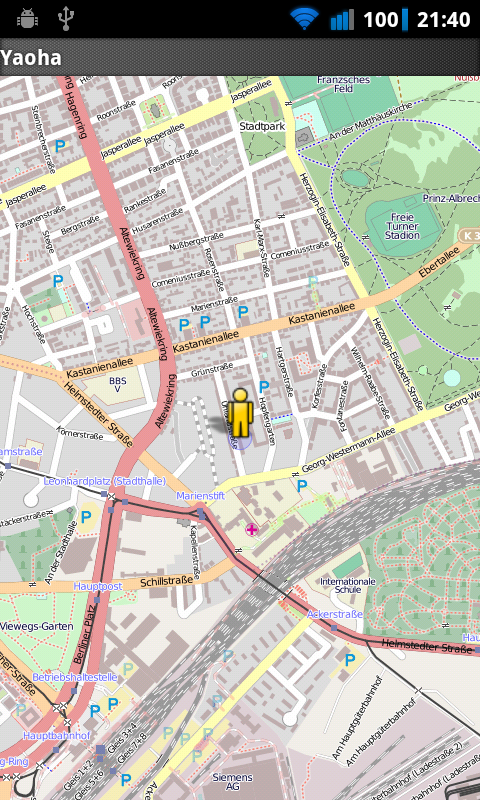
\includegraphics[scale=0.25]{map_plain.png}
  \end{columns}
\end{frame}

\begin{frame}
  \frametitle{Was wir bereits erreicht haben}
  \begin{columns}
  \column{5.1cm}
    \begin{itemize}
    \item Karten-view
    \alert<1>{\item Darstellen von Geschäften}
    \item Settings
    \item View für Suche
    \end{itemize}
  \column{5cm}
    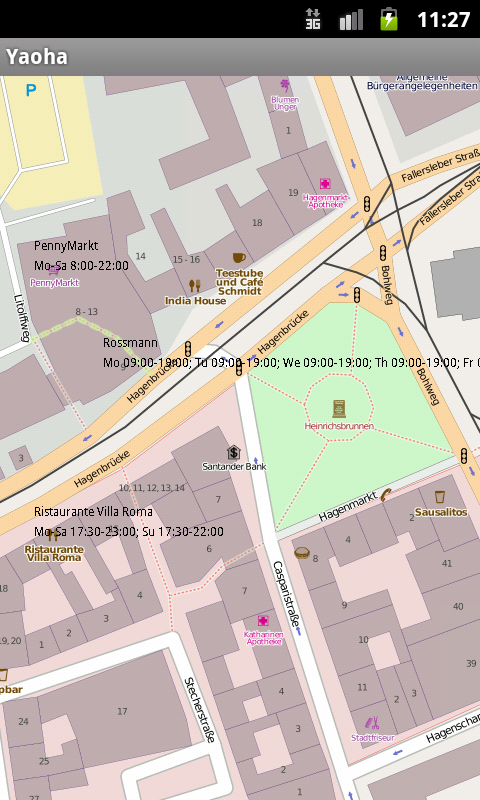
\includegraphics[scale=0.25]{map_shops3.png}
  \end{columns}
\end{frame}

\begin{frame}
  \frametitle{Was wir bereits erreicht haben}
  \begin{columns}
  \column{5.1cm}
    \begin{itemize}
    \item Karten-view
    \item Darstellen von Geschäften
    \alert<1>{\item Settings}
    \item View für Suche
    \end{itemize}
  \column{5cm}
    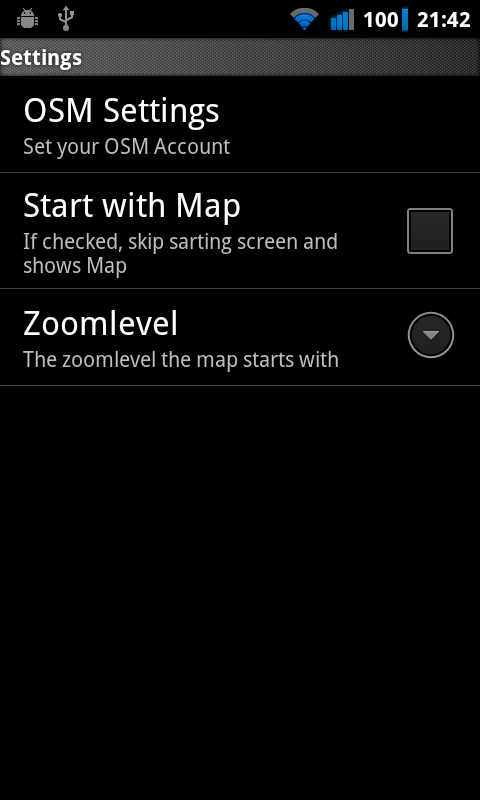
\includegraphics[scale=0.25]{settings1.png}
  \end{columns}
\end{frame}

\begin{frame}
  \frametitle{Was wir bereits erreicht haben}
  \begin{columns}
  \column{5.1cm}
    \begin{itemize}
    \item Karten-view
    \item Darstellen von Geschäften
    \item Settings
    \alert<1>{\item View für Suche}
    \end{itemize}
  \column{5cm}
    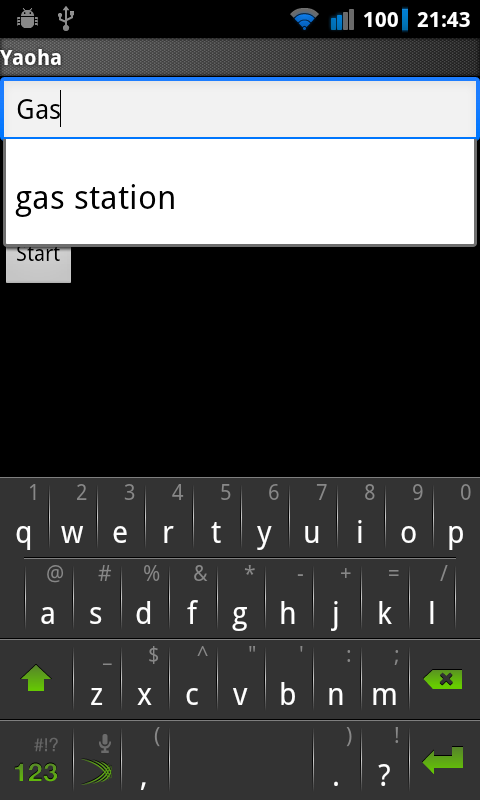
\includegraphics[scale=0.25]{search.png}
  \end{columns}
\end{frame}

\section{Probleme}
\frame{\frametitle{Outline} \tableofcontents[currentsection]}

\begin{frame}{Technische Probleme}
\begin{itemize}
\item Lokalisation nicht im Emulator testbar (Absturz)
\item Funktionen der Bibliothek zum Darstellen von OpenStreetMap haben leicht abweichendes Verhalten (Overlay)
\end{itemize}
\end{frame}

\begin{frame}{Organisatorische Probleme}
\begin{itemize}
\item Nicht immer klare Verteilung der Aufgaben (doppelte Arbeit)
\end{itemize}
\end{frame}

\end{document}
